\section{Introduction}

Being a huge fan of Matt and of Numperphile,
I recently watched the video \url{https://www.youtube.com/watch?v=q6L06pyt9CA},
featuring Matt Parker.  Despite Matt's infallibility, I decided to have my own
crack at the problem, in the spirit of mathematical enquiry and whatnot.

I reasoned that checking if a number is polygonal should be a roughly
\(\BigO(1)\) operation as we can find the \(n\)th term of the base-\(s\)
polygonal numbers \(P(s, n)\), which will be quadratic in \(n\), and solve it
for \(n\) with the quadratic formula, so to check if some cannonball numbers
\(C(s, n_c)\) is polygonal we just see if the corresponding \(n_p\) is an
integer. Now \(10^9\) is a fairly small number. Seeing as my CPU's clockspeed is
in the range of gigahertz, and we're just checking a tiny fraction of those
numbers as we're just computing the cannonball numbers under this limit, it
seems reasonable that this should be doable fairly fast.

I've thought about the problem of higher-dimensional stacks of cannonballs (ie
the ones formed by adding up the cannonball numbers), but I've not done anything
about it.

While I'm here I'd also like to plug square triangular numbers:
\url{https://en.wikipedia.org/wiki/Square_triangular_number}. I conjecture that
these are one of the least talked about, but coolest things in maths. For some
inexplicable reason (``````Pell's Equation''''''), if you take a convergent
\(b / c\) of \(\sqrt 2\), then \(b^2 c^2\) will be a square triangular number.
(Matt Parker voice) How cool is that?!

\section{State of the Union}

Below is presented a table of depths of \(s\) to which I've searched for various
upper bounds on \(C\). I did this mostly with one monumental overnight
computation on a fairly standard issue desktop computer (I can't bear to hear my
laptop's fan). Unfortunately I forgot to store the upper bound for each
computation, so they're just the largest number that's been found at that depth.
A couple of these may be an underestimate by about an order of magnitude.

\begin{longtable}{lr}
\toprule
\boldmath \(C(s, n) <\) & \boldmath \(s <\) \\
\midrule
\(10^{7}\) & 322 \\
\(10^{8}\) & 322 \\
\(10^{9}\) & 2378 \\
\(10^{10}\) & 2378 \\
\(10^{11}\) & 31265 \\
\(10^{12}\) & 31265 \\
\(10^{13}\) & 31265 \\
\(10^{18}\) & 223613 \\
\(10^{19}\) & 223613 \\
\(10^{20}\) & 223613 \\
\(10^{22}\) & 83135 \\
\(10^{24}\) & 9525 \\
\(10^{26}\) & 26 \\

\endhead
\bottomrule
\end{longtable}

I've also separately run some computation on numbers congruent to 2 module 3, as
I'll discuss more later. With these, I've checked polygons up the the gargantuan
103904-gon
.

\section{The Maths}

Indeed, this approach does seem to work. Almost by definition we have the
recurrence in polygonal numbers
\begin{equation*}
P(s, n) = P(s, n - 1) + n(s - 2) - (s - 3)
\end{equation*}
so we can use
\begin{align*}
P(s, n) &= \sum_{r = 1}^n P(s, r) - P(s, r - 1) \\
    &= \sum_{r = 1}^n (n(s - 2) - (s - 3)) \\
    &= \frac 12 n(n + 1)(s - 2) - n(s - 3) \\
    &= \frac{n^2(s - 2) - n(s - 4)} 2
\end{align*}
Fortunately this seems to agree with what Wikipedia thinks. Now, we have
\begin{alignat*}{2}
&& 0 &= (s - 2)n^2 - (s - 4)n - 2P(s, n) \\
&\implies& n &= \frac{s - 4 + \sqrt{(s - 4)^2 + 8(s - 2)P(s, n)}}{2s - 4}
\end{alignat*}
Wikipedia still seems to think we're on track.

Another result that I don't really use is that
\begin{align*}
C(s, n) &= \sum_{r = 1}^n P(s, n) \\
    &= \frac 12 \sum_{r = 1}^n (n^2(s - 2) - n(s - 4)) \\
    &= \frac 12 \pqty{\frac{n(n + 1)(2n + 1)(s - 2)} 6
                    - \frac{n(n + 1)(s - 4)} 2} \\
    &= \frac 1{12}n(n + 1)\bqty{(2n + 1)(s - 2) - 3(s - 4)}
\end{align*}
In fact I've only used this in verification of the results.

Regardless, now we need only work our way up the \(C(s, n)\)s using the
recurrence \(C(s, n) = P(s, n) + C(s, n - 1)\), and check for each if the
quadratic formula gives an integer result. This is most easily done by checking
if the discriminant is a perfect square and then checking that the denominator
divides the numerator.

Later on I experimentally determined some formulae that give an integer solution
for any \(s \equiv 2 \pmod 3\).
\begin{align*}
n_P &= \tfrac 19s^3 - \tfrac 23s^2 + \tfrac 13s + \tfrac{19}9 \\
n_C &= \tfrac 13s^2 - \tfrac 43s - \tfrac 23 \\
C &= \tfrac{1}{162}s^7 - \tfrac{7}{81}s^6 + \tfrac{11}{27}s^5 - \tfrac{91}{162}s^4
    - \tfrac{133}{162}s^3 + \tfrac{103}{54}s^2 + \tfrac{35}{81}s - \tfrac{19}{81}
\end{align*}
It can be verified by some fairly gruesome (computer assisted - listing
\ref{lst_sympy_alg}) algebra, letting \(s = 3k+2\) and substituting into the
formulae given above, that this result works.
\begin{align*}
n_P &= k + \frac{\left(3 k + 2\right)^{3}}{9} - \frac{2 \left(3 k + 2\right)^{2}}{3} + \frac{25}{9} \\
    &= 3 k^{3} - 3 k + 1 \\
n_C &= - 4 k + \frac{\left(3 k + 2\right)^{2}}{3} - \frac{10}{3} \\
    &= 3 k^{2} - 2 \\
P(s, n_P) &= - \frac{\left(s - 4\right) \left(\frac{s^{3}}{9} - \frac{2 s^{2}}{3} + \frac{s}{3} + \frac{19}{9}\right)}{2} + \frac{\left(s - 2\right) \left(\frac{s^{3}}{9} - \frac{2 s^{2}}{3} + \frac{s}{3} + \frac{19}{9}\right)^{2}}{2} \\[3ex]
          &= \frac{s^{7}}{162} - \frac{7 s^{6}}{81} + \frac{11 s^{5}}{27} - \frac{91 s^{4}}{162} - \frac{133 s^{3}}{162} + \frac{103 s^{2}}{54} + \frac{35 s}{81} - \frac{19}{81} \\[3ex]
C(s, n_C) &= \frac{\left(- 3 s + \left(s - 2\right) \left(\frac{2 s^{2}}{3} - \frac{8 s}{3} - \frac{1}{3}\right) + 12\right) \left(\frac{s^{2}}{3} - \frac{4 s}{3} - \frac{2}{3}\right) \left(\frac{s^{2}}{3} - \frac{4 s}{3} + \frac{1}{3}\right)}{12} \\[3ex]
          &= \frac{s^{7}}{162} - \frac{7 s^{6}}{81} + \frac{11 s^{5}}{27} - \frac{91 s^{4}}{162} - \frac{133 s^{3}}{162} + \frac{103 s^{2}}{54} + \frac{35 s}{81} - \frac{19}{81}
\end{align*}
(I have shown here that \(n_C\) and \(n_P\) are both integers, and that the
formulae for \(P(s, n_P)\) and \(C(s, n_C)\) give the same result))

It still remains utterly beyond my comprehension as to where this formula comes
from, or how to determine if there are more like it. Really I don't have enough
data points to extrapolate any more seventh-degree polynomials, but the chances
are they'd be much larger.

\begin{longlisting}
\begin{minted}{python}
s, k = symbols("s k")
P = lambda s, n: (n ** 2 * (s - 2) - n * (s - 4)) / 2
C = lambda s, n: n * (n + 1) * ((2 * n + 1) * (s - 2) - 3 * (s - 4)) / 12
n_P = s ** 3 / 9 - 2 * s ** 2 / 3 + s / 3 + S(19) / 9
n_C = s ** 2 / 3 - 4 * s / 3 - S(2) / 3
print(r"n_P &= {} \\".format(latex(n_P.subs(s, 3 * k + 2))))
print(r"    &= {} \\".format(latex(simplify(n_P.subs(s, 3 * k + 2)))))
print(r"n_C &= {} \\".format(latex(n_C.subs(s, 3 * k + 2))))
print(r"    &= {} \\".format(latex(simplify(n_C.subs(s, 3 * k + 2)))))
print(r"P(s, n_P) &= {} \\[3ex]".format(latex(P(s, n_P))))
print(r"          &= {} \\[3ex]".format(latex(simplify(P(s, n_P)))))
print(r"C(s, n_C) &= {} \\[3ex]".format(latex(C(s, n_C))))
print(r"          &= {}".format(latex(simplify(C(s, n_C)))))
\end{minted}
\caption{Doing algebra}\label{lst_sympy_alg}
\end{longlisting}

\section{The Programming}

For speeeeeeed I implemented this in C (although there is a long abandoned
parallel Python implementation). I used 128-bit integers to be on the safe side,
as \(10^{19}\) is a little small for my liking. This meant I had to do a lot of
messing around to get things to actually display in base 10. This program is
shown in Listing \ref{lst_c}.

Of course, an isolated source code listing is both not executable and not
necessarily helpful, but fret not as my intact source tree is in
\texttt{../src}.

I did briefly consider either implementing or importing some kind of arbitrary
precision integer arithmetic functionality, but then I decided I wasn't going to
run it on anything fast enough to have to worry about that, and I have better
things to do.

There's also a slick little progress update that gets printed to STDERR. I've
written a number of interacting zsh scripts and Python scripts here and there to
manage the actual programs, forming a sort of terribly managed little pipeline,
with files that don't make any sense all over the place. Much of it is probably
also dependent on software that happens to be on my computer, like some Linux
coreutils. Obviously the C code will probably require GCC to work out of the
box.

I also have a program that verifies results, removes duplicates and formats them
into a \LaTeX{} table (spoilers for table \ref{tab_ugly}), shown in listing
\ref{lst_py_verif}.

After having used these programs to obtain some data, and plot it and so on and
so forth as discussed in the next section, I noticed the glaring pattern with
the cannonball numbers derived from a side congruent to 2 modulo 3. By
assuming that this pattern continues, in that you can move 3 along and a little
up to get to a new cannonball polygonal number, it is easy to generate these
kinds of numbers at a preposterous rate. I wrote a little C program (listing
\ref{lst_c_2mod3} which took maybe ten minutes to hit the upper bounds of
128-bit integer arithmetic, getting me to around 80000.

I then wrote a Python program (listing \ref{lst_py_2mod3}), which was at first
just a straightforward translation, to take advantage of Python's arbitrary
precision integers. I then decided I could probably take further advantage of
the curve, because really going up in linear steps felt a bit slow. I assumed
that the graph of \(s\) against \(n_C\) would be convex, such that each gap
between numbers is greater than the last. By making this assumption, I suddenly
started generating tens of thousands of solutions per second, getting to the
point where IO is the main bottleneck.

\begin{longlisting}
\inputminted{c}{../src/c/cannonball.c}
\caption{The main C source code}
\label{lst_c}
\end{longlisting}

\begin{longlisting}
\inputminted{python}{../src/factcheck.py}
\caption{Python verification program}
\label{lst_py_verif}
\end{longlisting}

\begin{longlisting}
\inputminted{c}{../src/c/2mod3/2mod3.c}
\caption{C program to find cannonball polygons for side congruent to 2 mod 3}
\label{lst_c_2mod3}
\end{longlisting}

\begin{longlisting}
\inputminted{python}{../src/c/2mod3/2mod3.py}
\caption{Python program like (\ref{lst_c_2mod3}) but cleverer.}
\label{lst_py_2mod3}
\end{longlisting}

\section{The Ugly}

I have plotted both the data in its entirety on a double logarithmic scale
\ref{fig_log_all}. The graphs started becoming so large after I came up with the
trick to generate 2-mod-3 numbers that I had to rasterise them. You can modify
the R code to make them be PDFs if you want but it will be slow.

The obvious pattern that jumps out is the big line of points for all the sides
congruent to \(2 \pmod 3\). Particularly because it looks like such a straight
line on the log-log plot, we would expect it to be modelled well as a constant
multiple of some power of \(s\). I drew two lines that seemed to roughly bound
it, and used those to extract the points on the line and then do some linear
regression on that (figure \ref{fig_log_boring}). I obtained the formula
\begin{equation*}
C = 0.006170169 \cdot s ^ { 7.000026 }
\qquad \text{Average percentage error of  0.001840273 \%}\end{equation*}

This would seem to imply to me that it's probably a seventh-degree polynomial.

I wrote this paragraph, but not for a very long time did I think to actually
check. I first wasted a lot of time trying to brute force more points on the
line. When I did decide to check, I wrote the little Python program in listing
\ref{lst_sympy}, using the library Sympy to do a little linear algebra. I had a
sample of points from the line, from which I sampled randomly as a poor
approximation to checking if the fit works for all points. However, much to my
surprise, the program did consistently output the same coefficients, indicating
that the general formula for \(C\) where \(s \equiv 2 \pmod 3\) is (probably)
\begin{equation*}
C = \tfrac{1}{162}s^7 - \tfrac{7}{81}s^6 + \tfrac{11}{27}s^5 - \tfrac{91}{162}s^4
    - \tfrac{133}{162}s^3 + \tfrac{103}{54}s^2 + \tfrac{35}{81}s - \tfrac{19}{81}
\end{equation*}

I also used a similar approach to calculate a cubic and quadratic formula for
\(n_P\) and \(n_C\) in terms of \(s\).
%Matrix([[1/162], [-7/81], [11/27], [-91/162], [-133/162], [103/54], [35/81], [-19/81]])
%Matrix([[1/9], [-2/3], [1/3], [19/9]])
%Matrix([[1/3], [-4/3], [-2/3]])
\begin{align*}
n_P &= \tfrac 19s^3 - \tfrac 23s^2 + \tfrac 13s + \tfrac{19}9 \\
n_C &= \tfrac 13s^2 - \tfrac 43s - \tfrac 23
\end{align*}

I used this expression to calculate a really big number just for the hell of it.
I wrote a little code (as seen in listing \ref{lst_infinity}) to take some
integer \(i_n\), calculate \(s_n = 3i_n + 2\) and \(C_n\) from there. Now I made
repeatedly square \(i_n\) to advance - ie \(i_{n + 1} = i_n^2\) - just to
quickly get very big numbers. In fact I found that almost all of the hard bit is
calculating base-10 representations and typesetting them. \LaTeX{} very quickly
crashes with the biggest numbers I found (see
\texttt{../infinity\_and\_beyond/solutions/}), so I settled on a smaller one.
I used a sequence of \(9\) just because I wanted to use \(10\)s, but they end up
looking really artificial, because when you have a polynomial in a power of 10
you get odd artifacts in base 10.

\begin{longlisting}
\inputminted{python}{../investigate/solve.py}
\caption{Trying to find a polynomial}
\label{lst_sympy}
\end{longlisting}

\begin{longlisting}
\inputminted{python}{../infinity_and_beyond/buzz.py}
\caption{Calculating big numbers because I can}
\label{lst_infinity}
\end{longlisting}

I have also plotted these points on a linear scale, demonstrating their
relationship \ref{fig_linear_boring}.

Lastly, I plotted all points other than the points along this line in figure
\ref{fig_log_interesting}.

The R code I used to achieve all this is in Listing \ref{lst_R}.

Table \ref{tab_ugly} lists some solutions that I've found, so far. The \TeX{}
source of the table is in \texttt{../graph/interesting.tsv}, which is derived
from \texttt{../src/c/solutions/*}.  I have deliberately omitted the ``boring''
solutions along the dense line, favouring the more flavourful, stylish and
individualistic solutions.

There are also two tables \texttt{boring.tsv} and \texttt{all.tsv} containing
only the boring solutions and all solutions, respectively, but there are such a
truly mind-boggling number of boring solutions that really it's hardly any fun
looking at them.

Unfortunately at this point they're so big that I've had to arbitraryily curtail
them to 10000 lines, presented in \texttt{all\_extract.tsv}. The full length of
\texttt{all.tsv} is currently  12536693 all.tsv
.

The rate of generation of these solutions is several orders of
magnitude above anything else, which does mean that you should be able to
generate your own set of a couple hundred million fairly quickly.

I have presented an extract of the full data set in the document
\texttt{biglist.pdf}.

\begin{longlisting}
\inputminted{R}{../graph/graph.R}
\caption{R graphical analysis}
\label{lst_R}
\end{longlisting}

\begin{figure}[H]
\centering
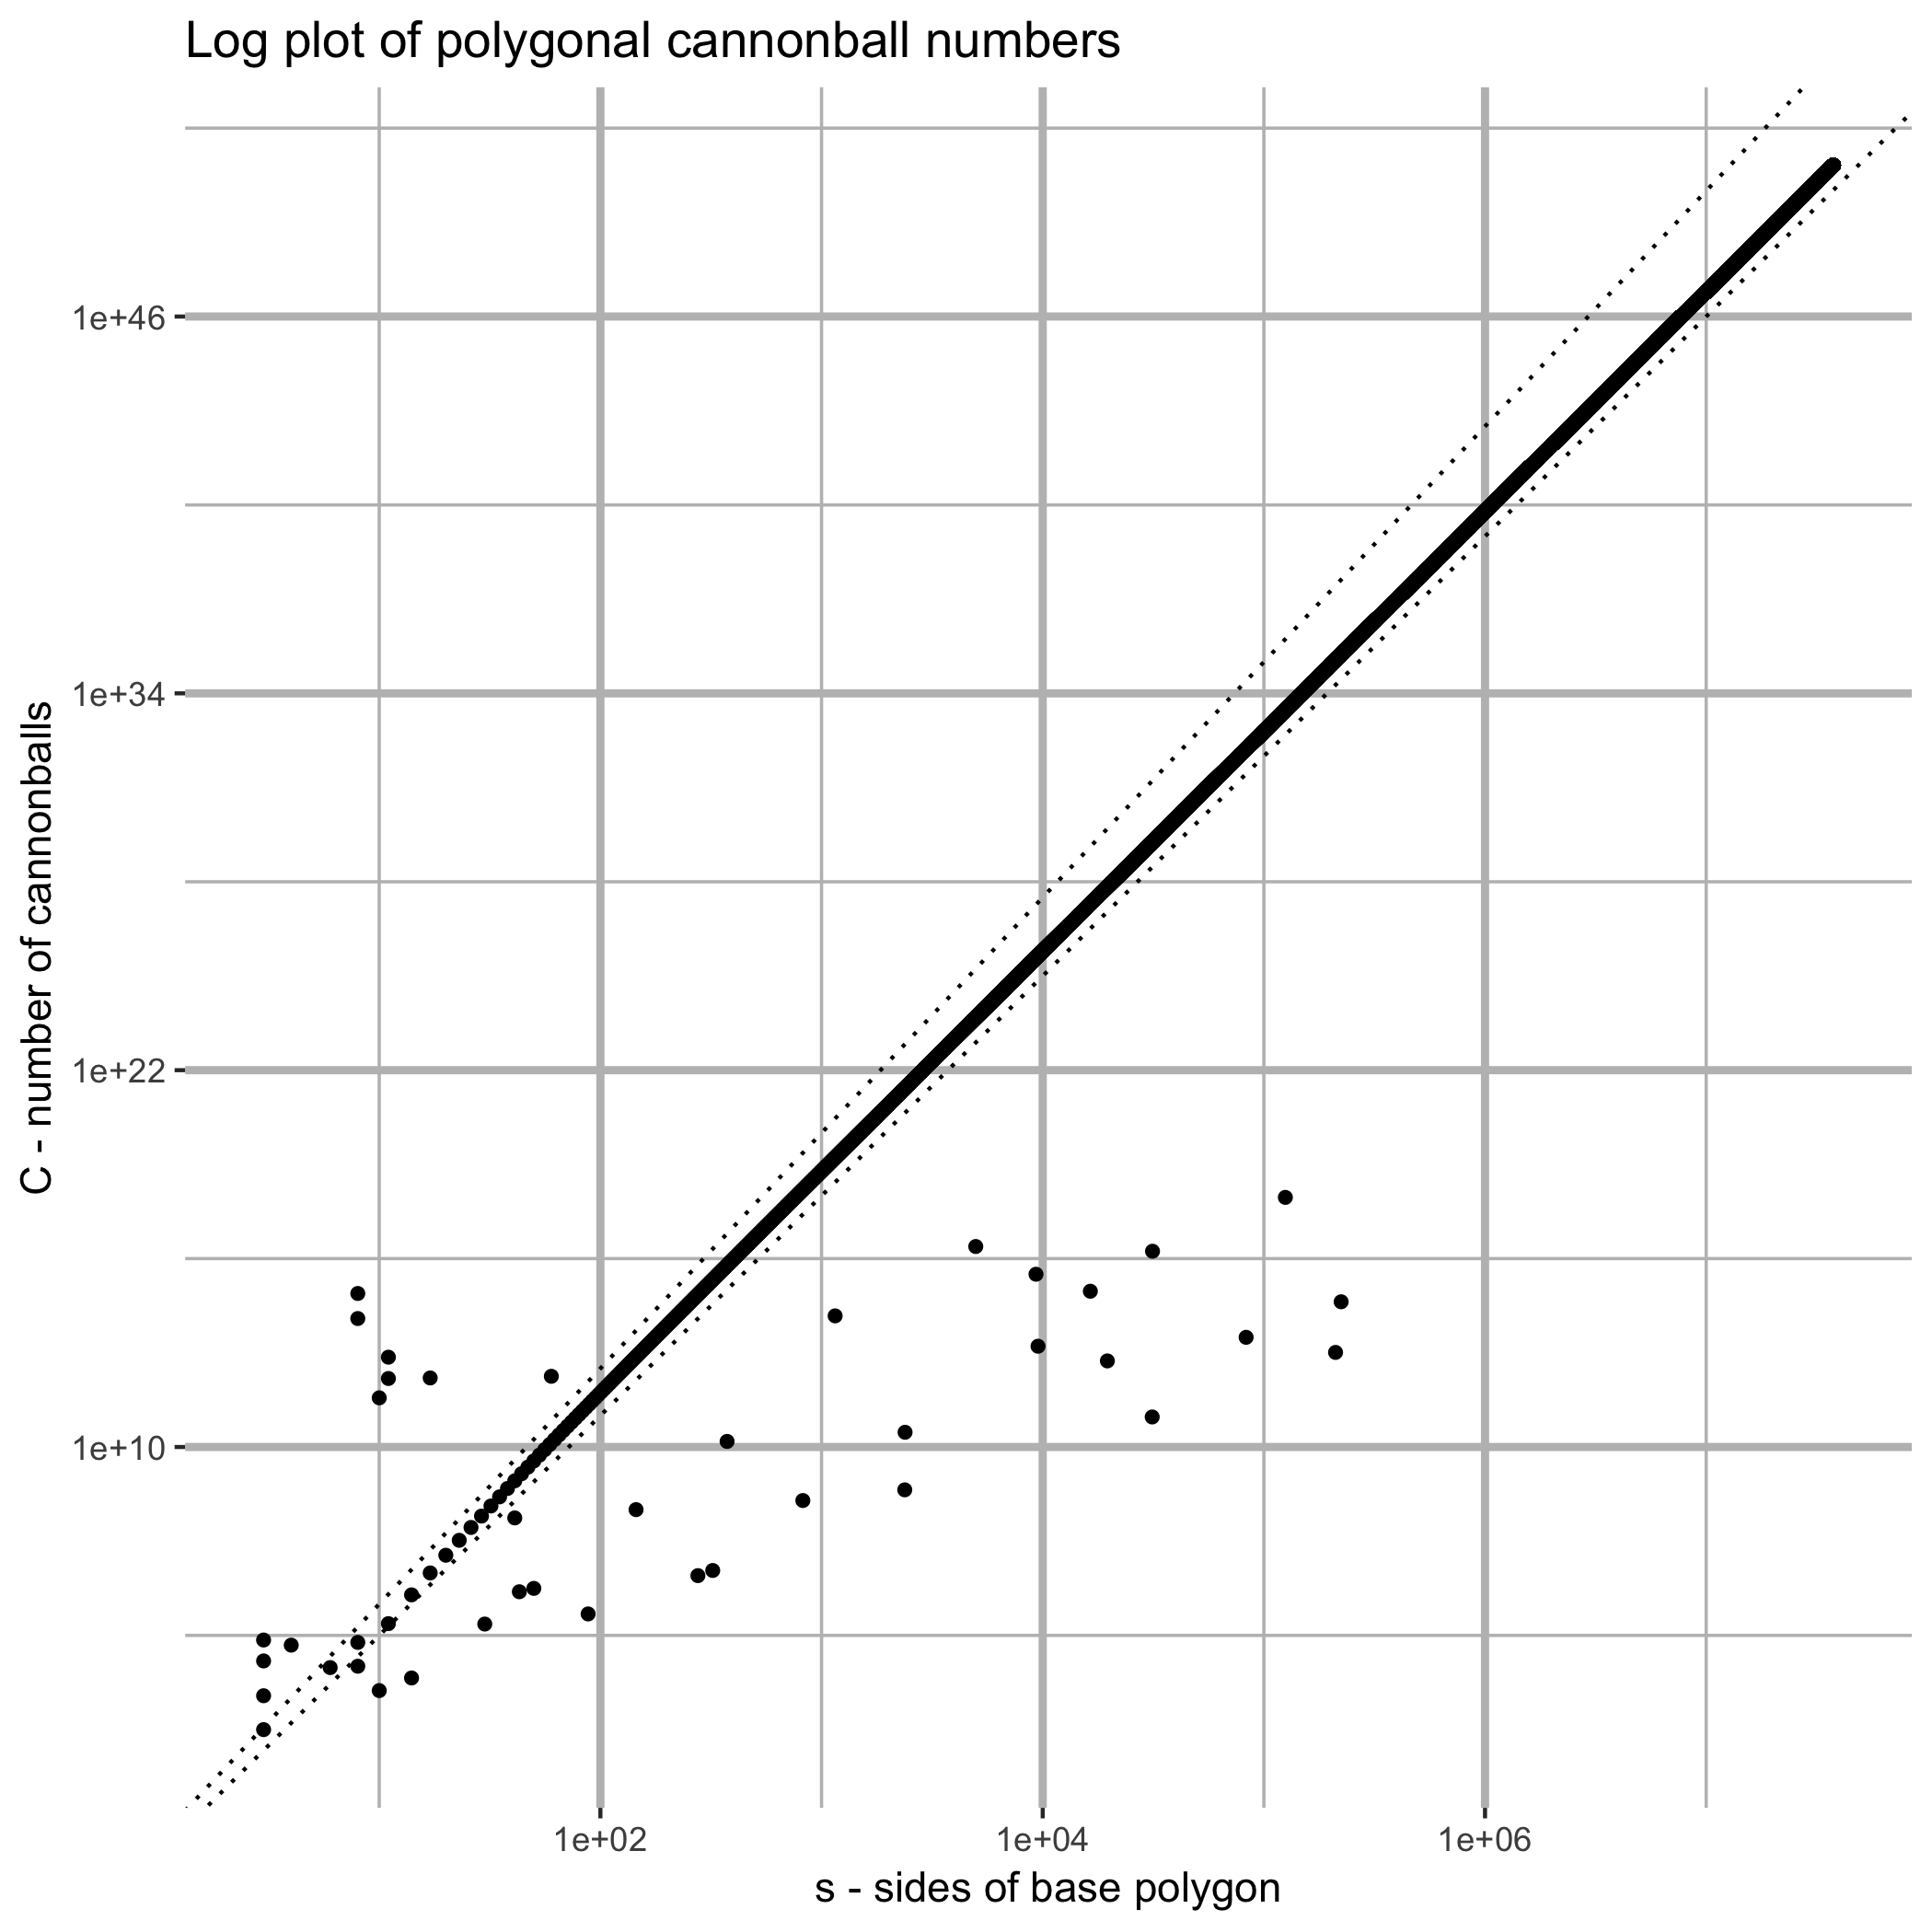
\includegraphics[width=\textwidth]{../graph/all_log.png}
\caption{Log plot}
\label{fig_log_all}
\end{figure}

\begin{figure}[H]
\centering
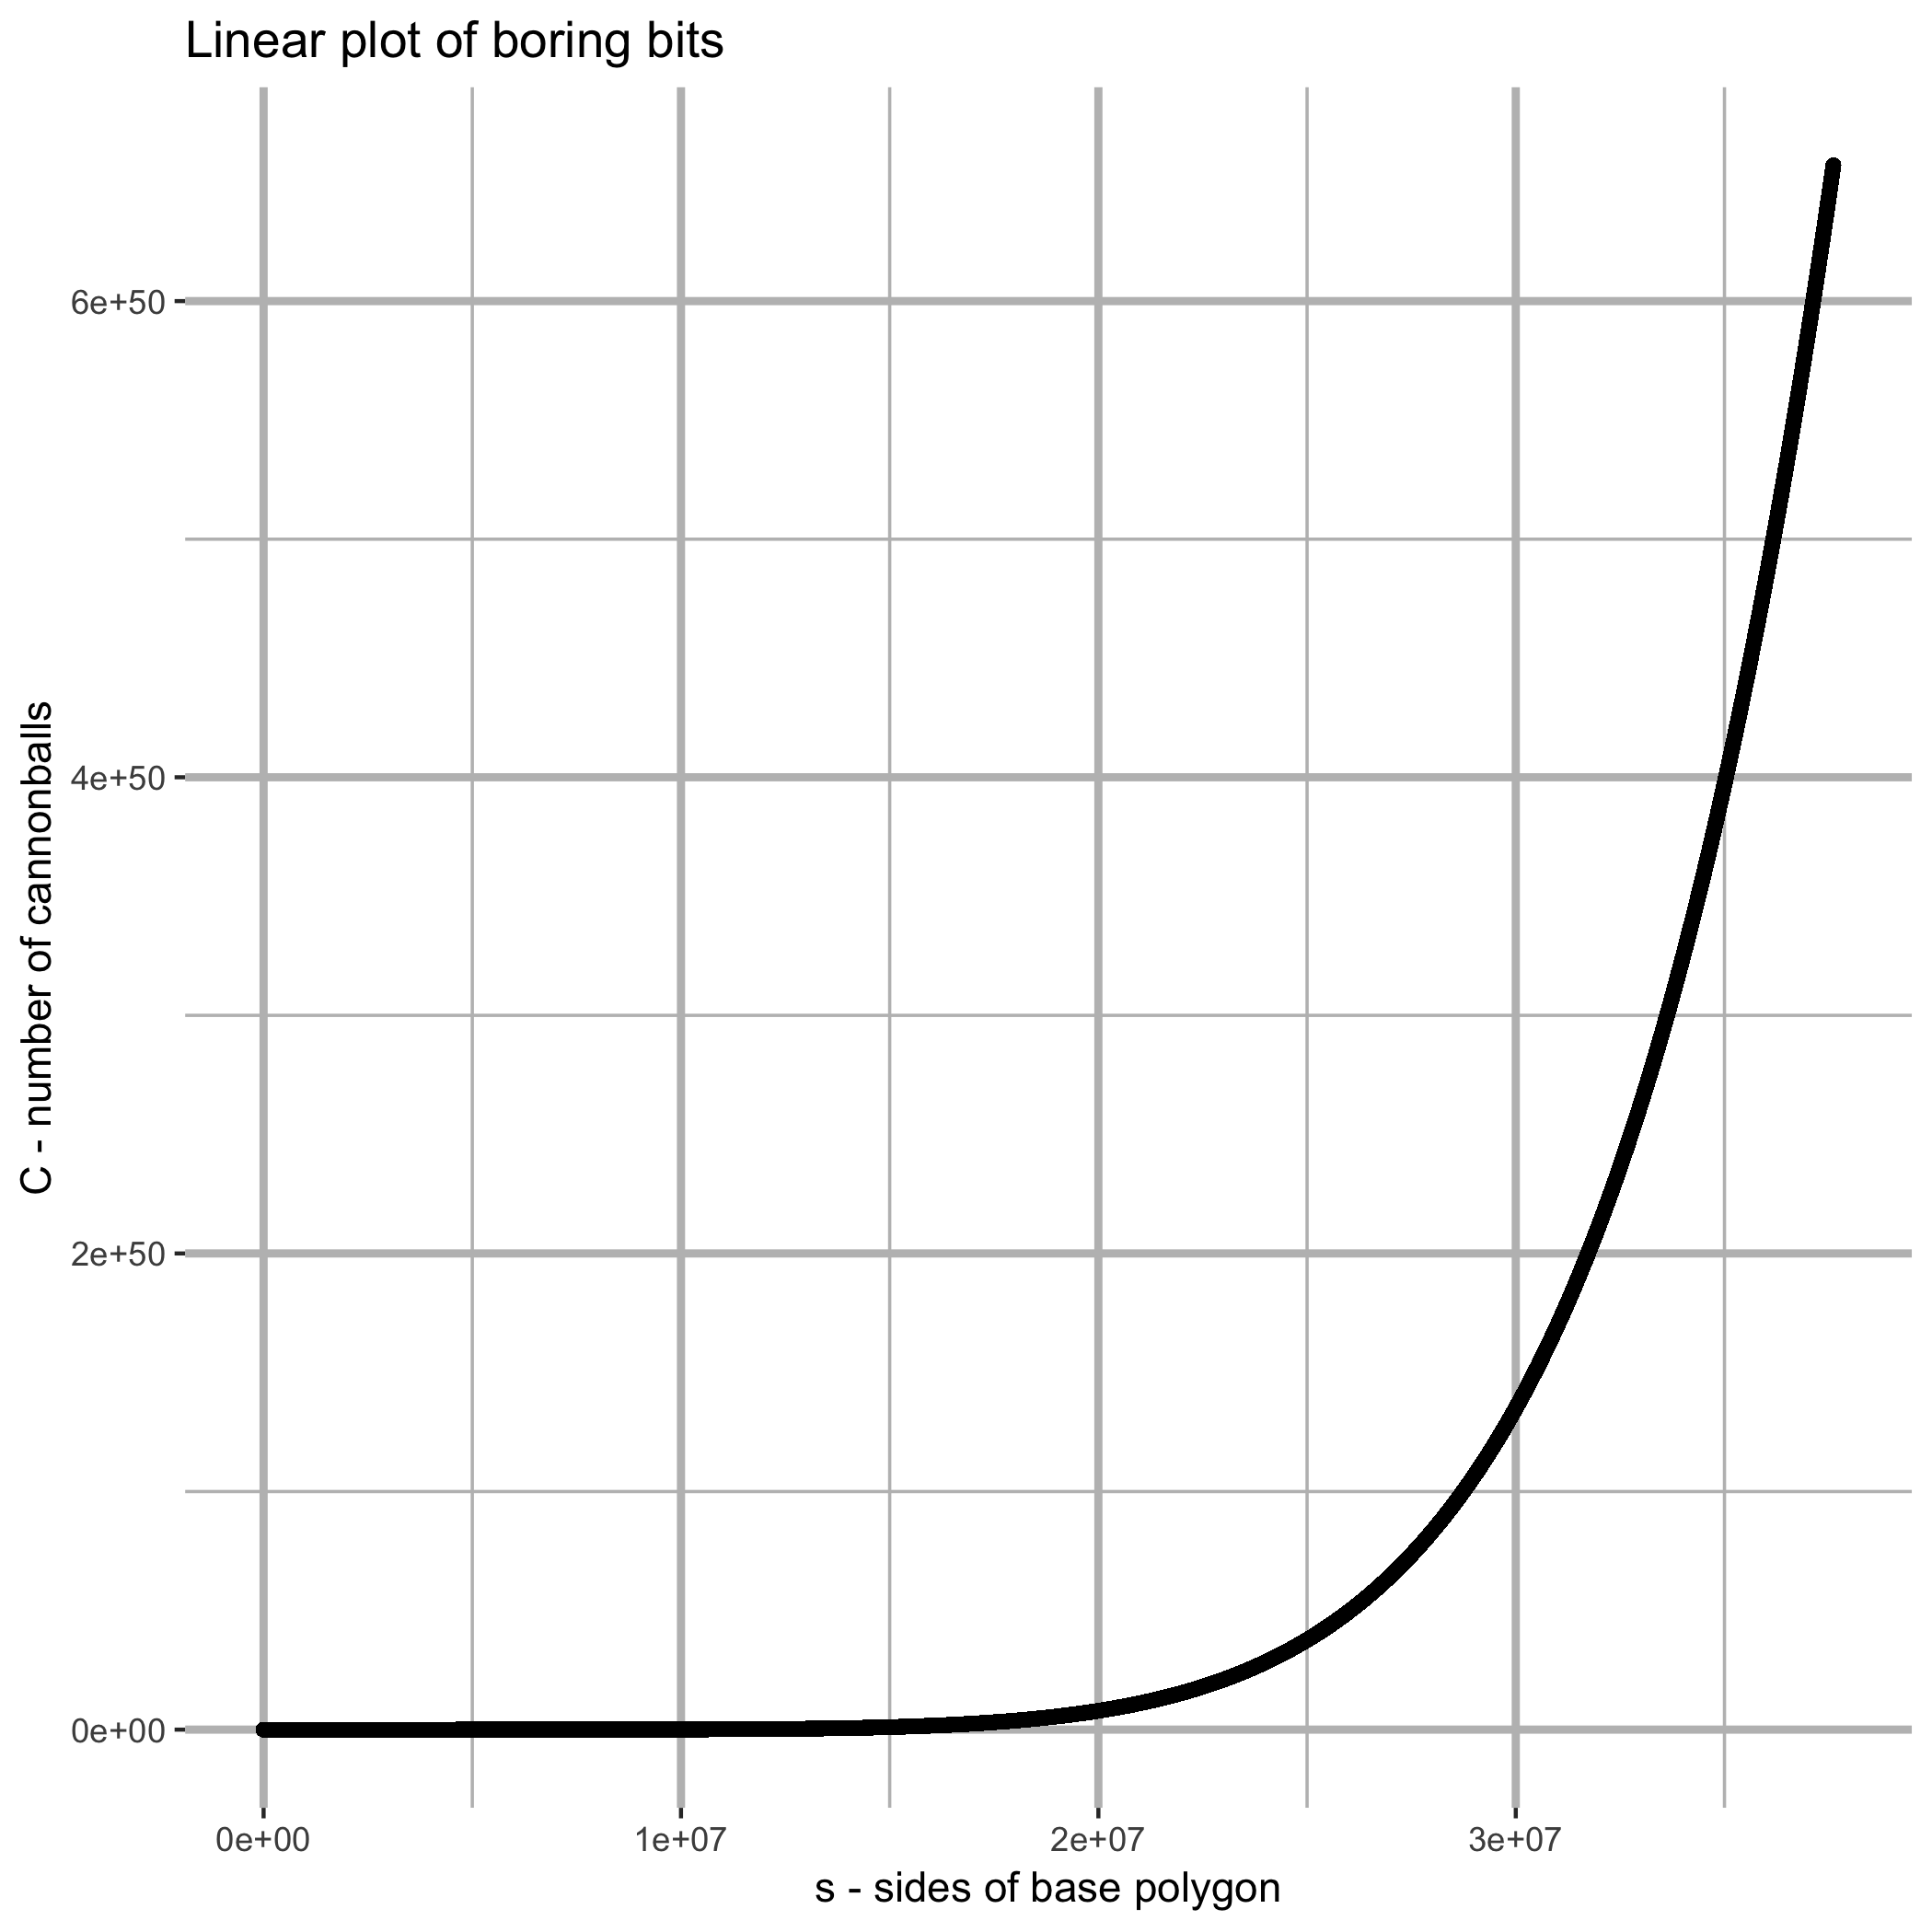
\includegraphics[width=\textwidth]{../graph/boring_lin.png}
\caption{Linear plot of boring points}
\label{fig_linear_boring}
\end{figure}

\begin{figure}[H]
\centering
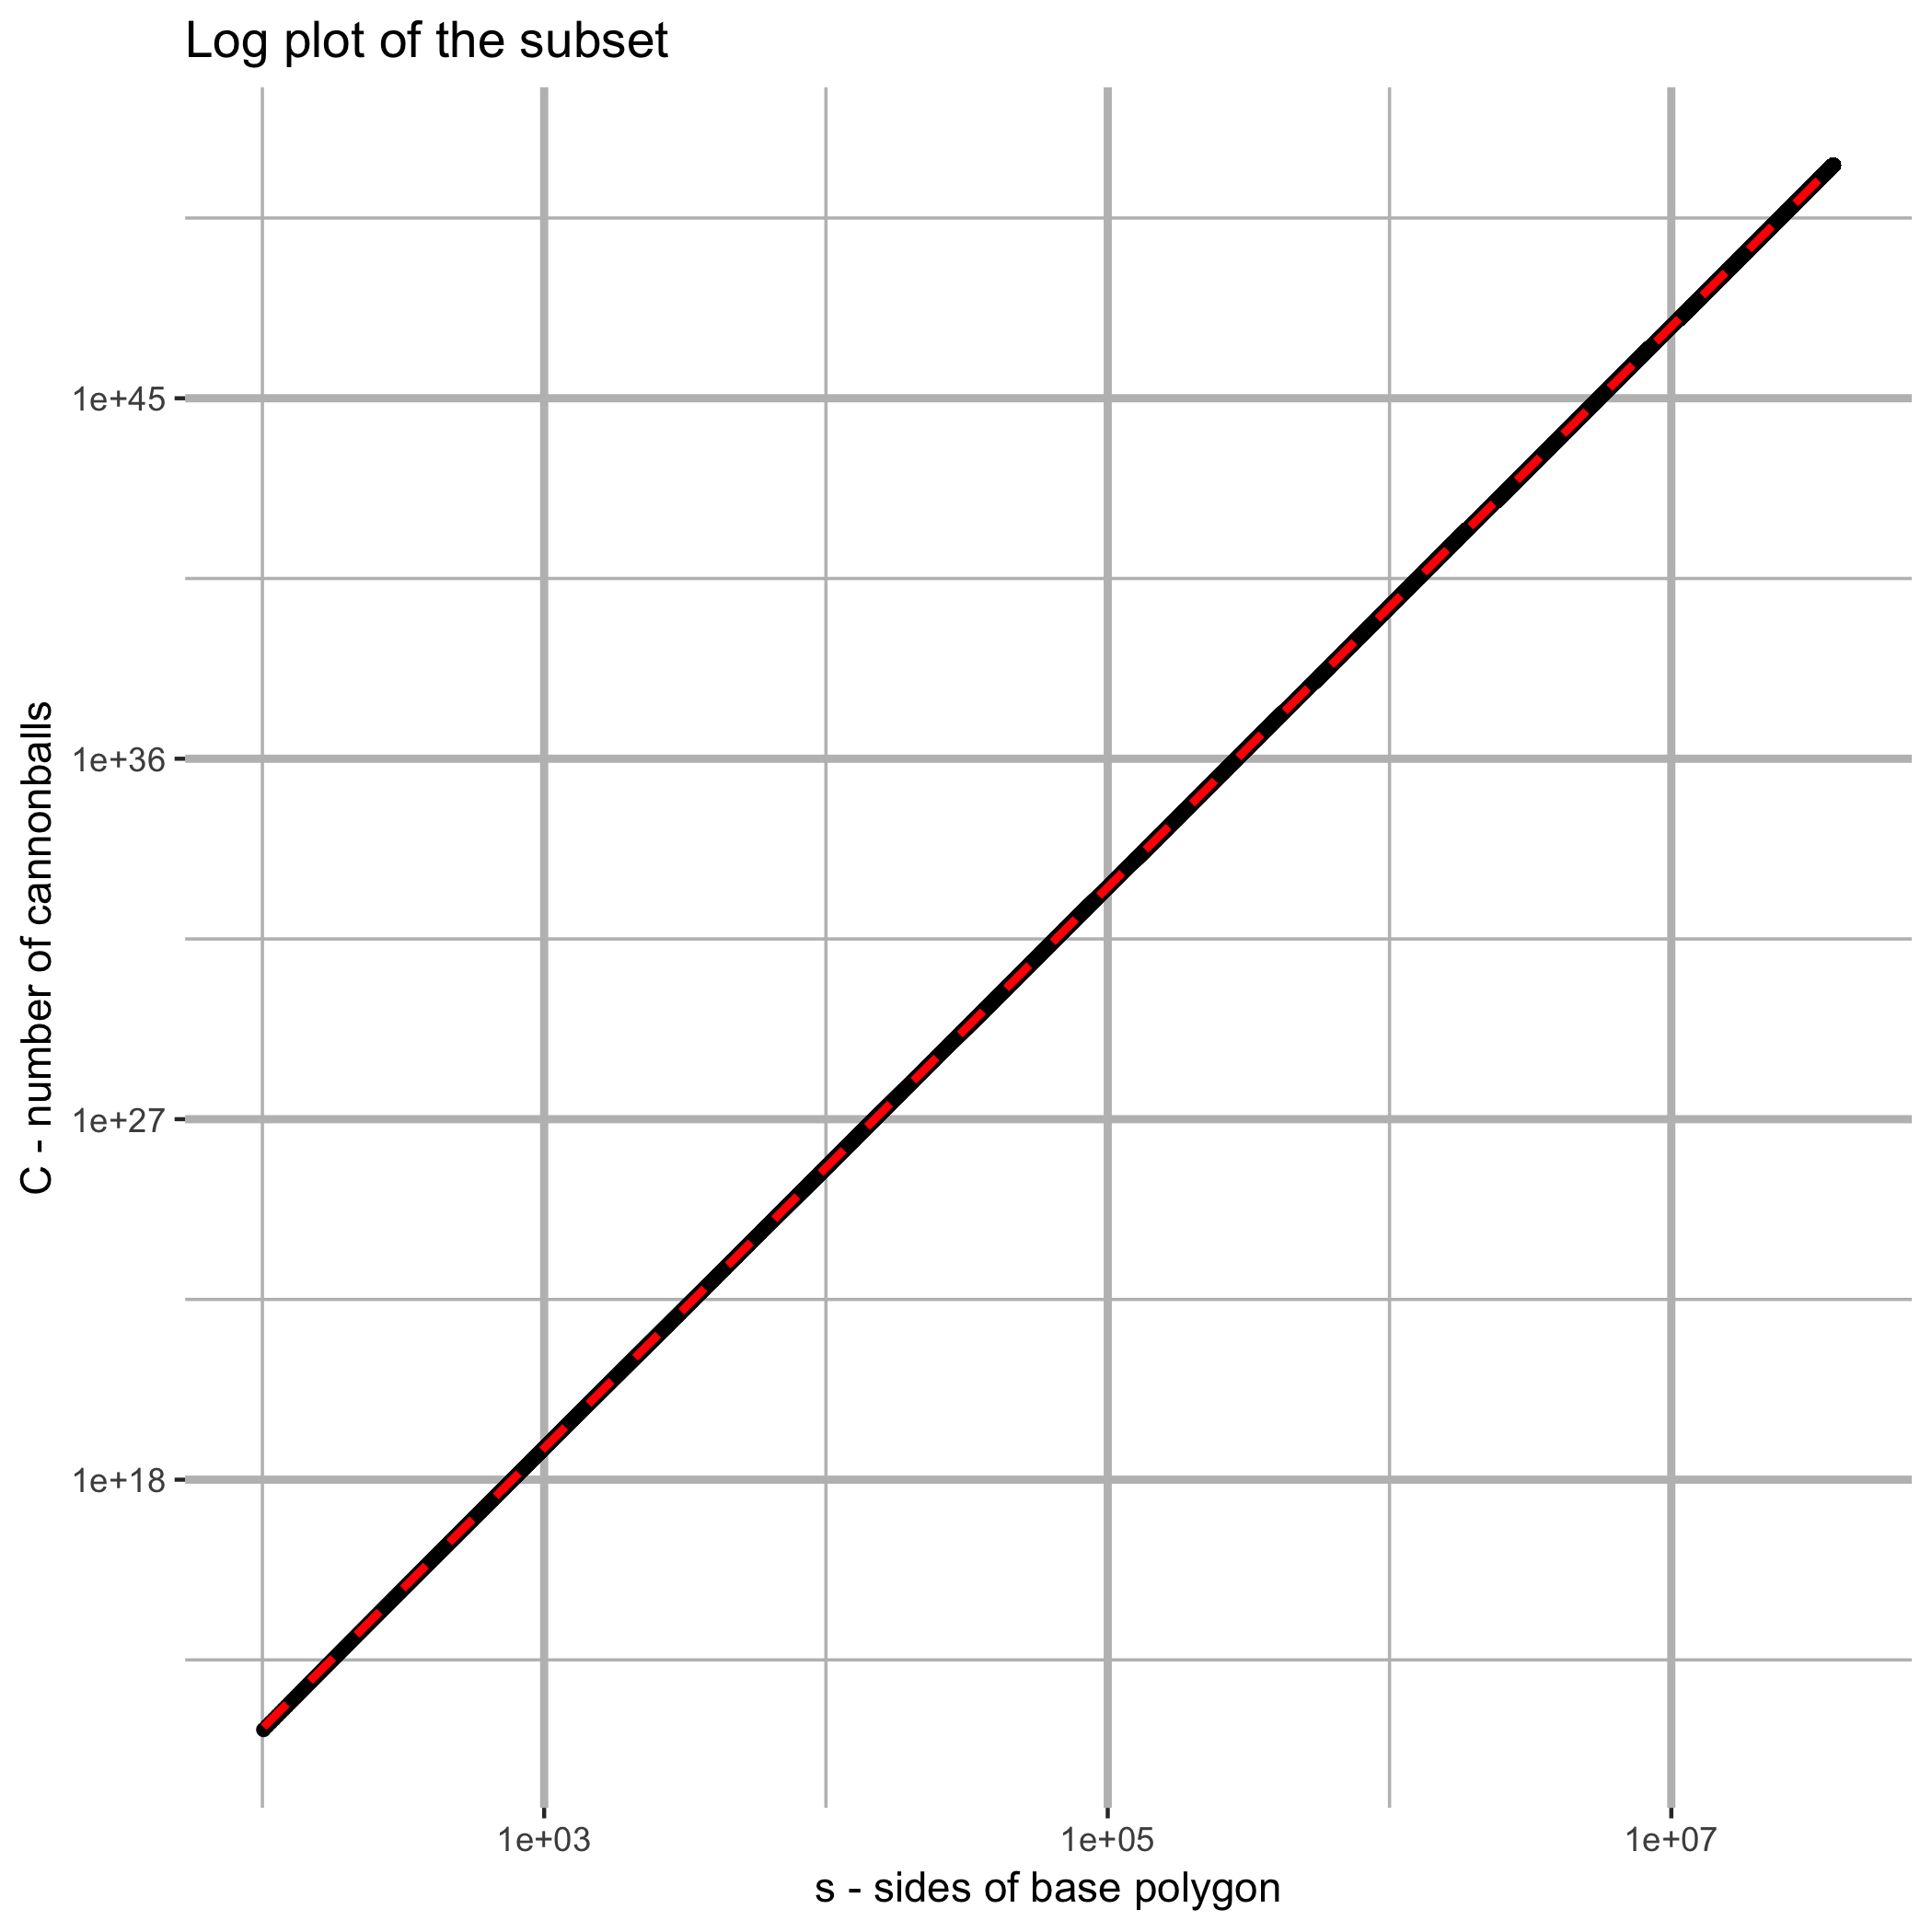
\includegraphics[width=\textwidth]{../graph/boring_log.png}
\caption{Log plot of the boring points}
\label{fig_log_boring}
\end{figure}

\begin{figure}[H]
\centering
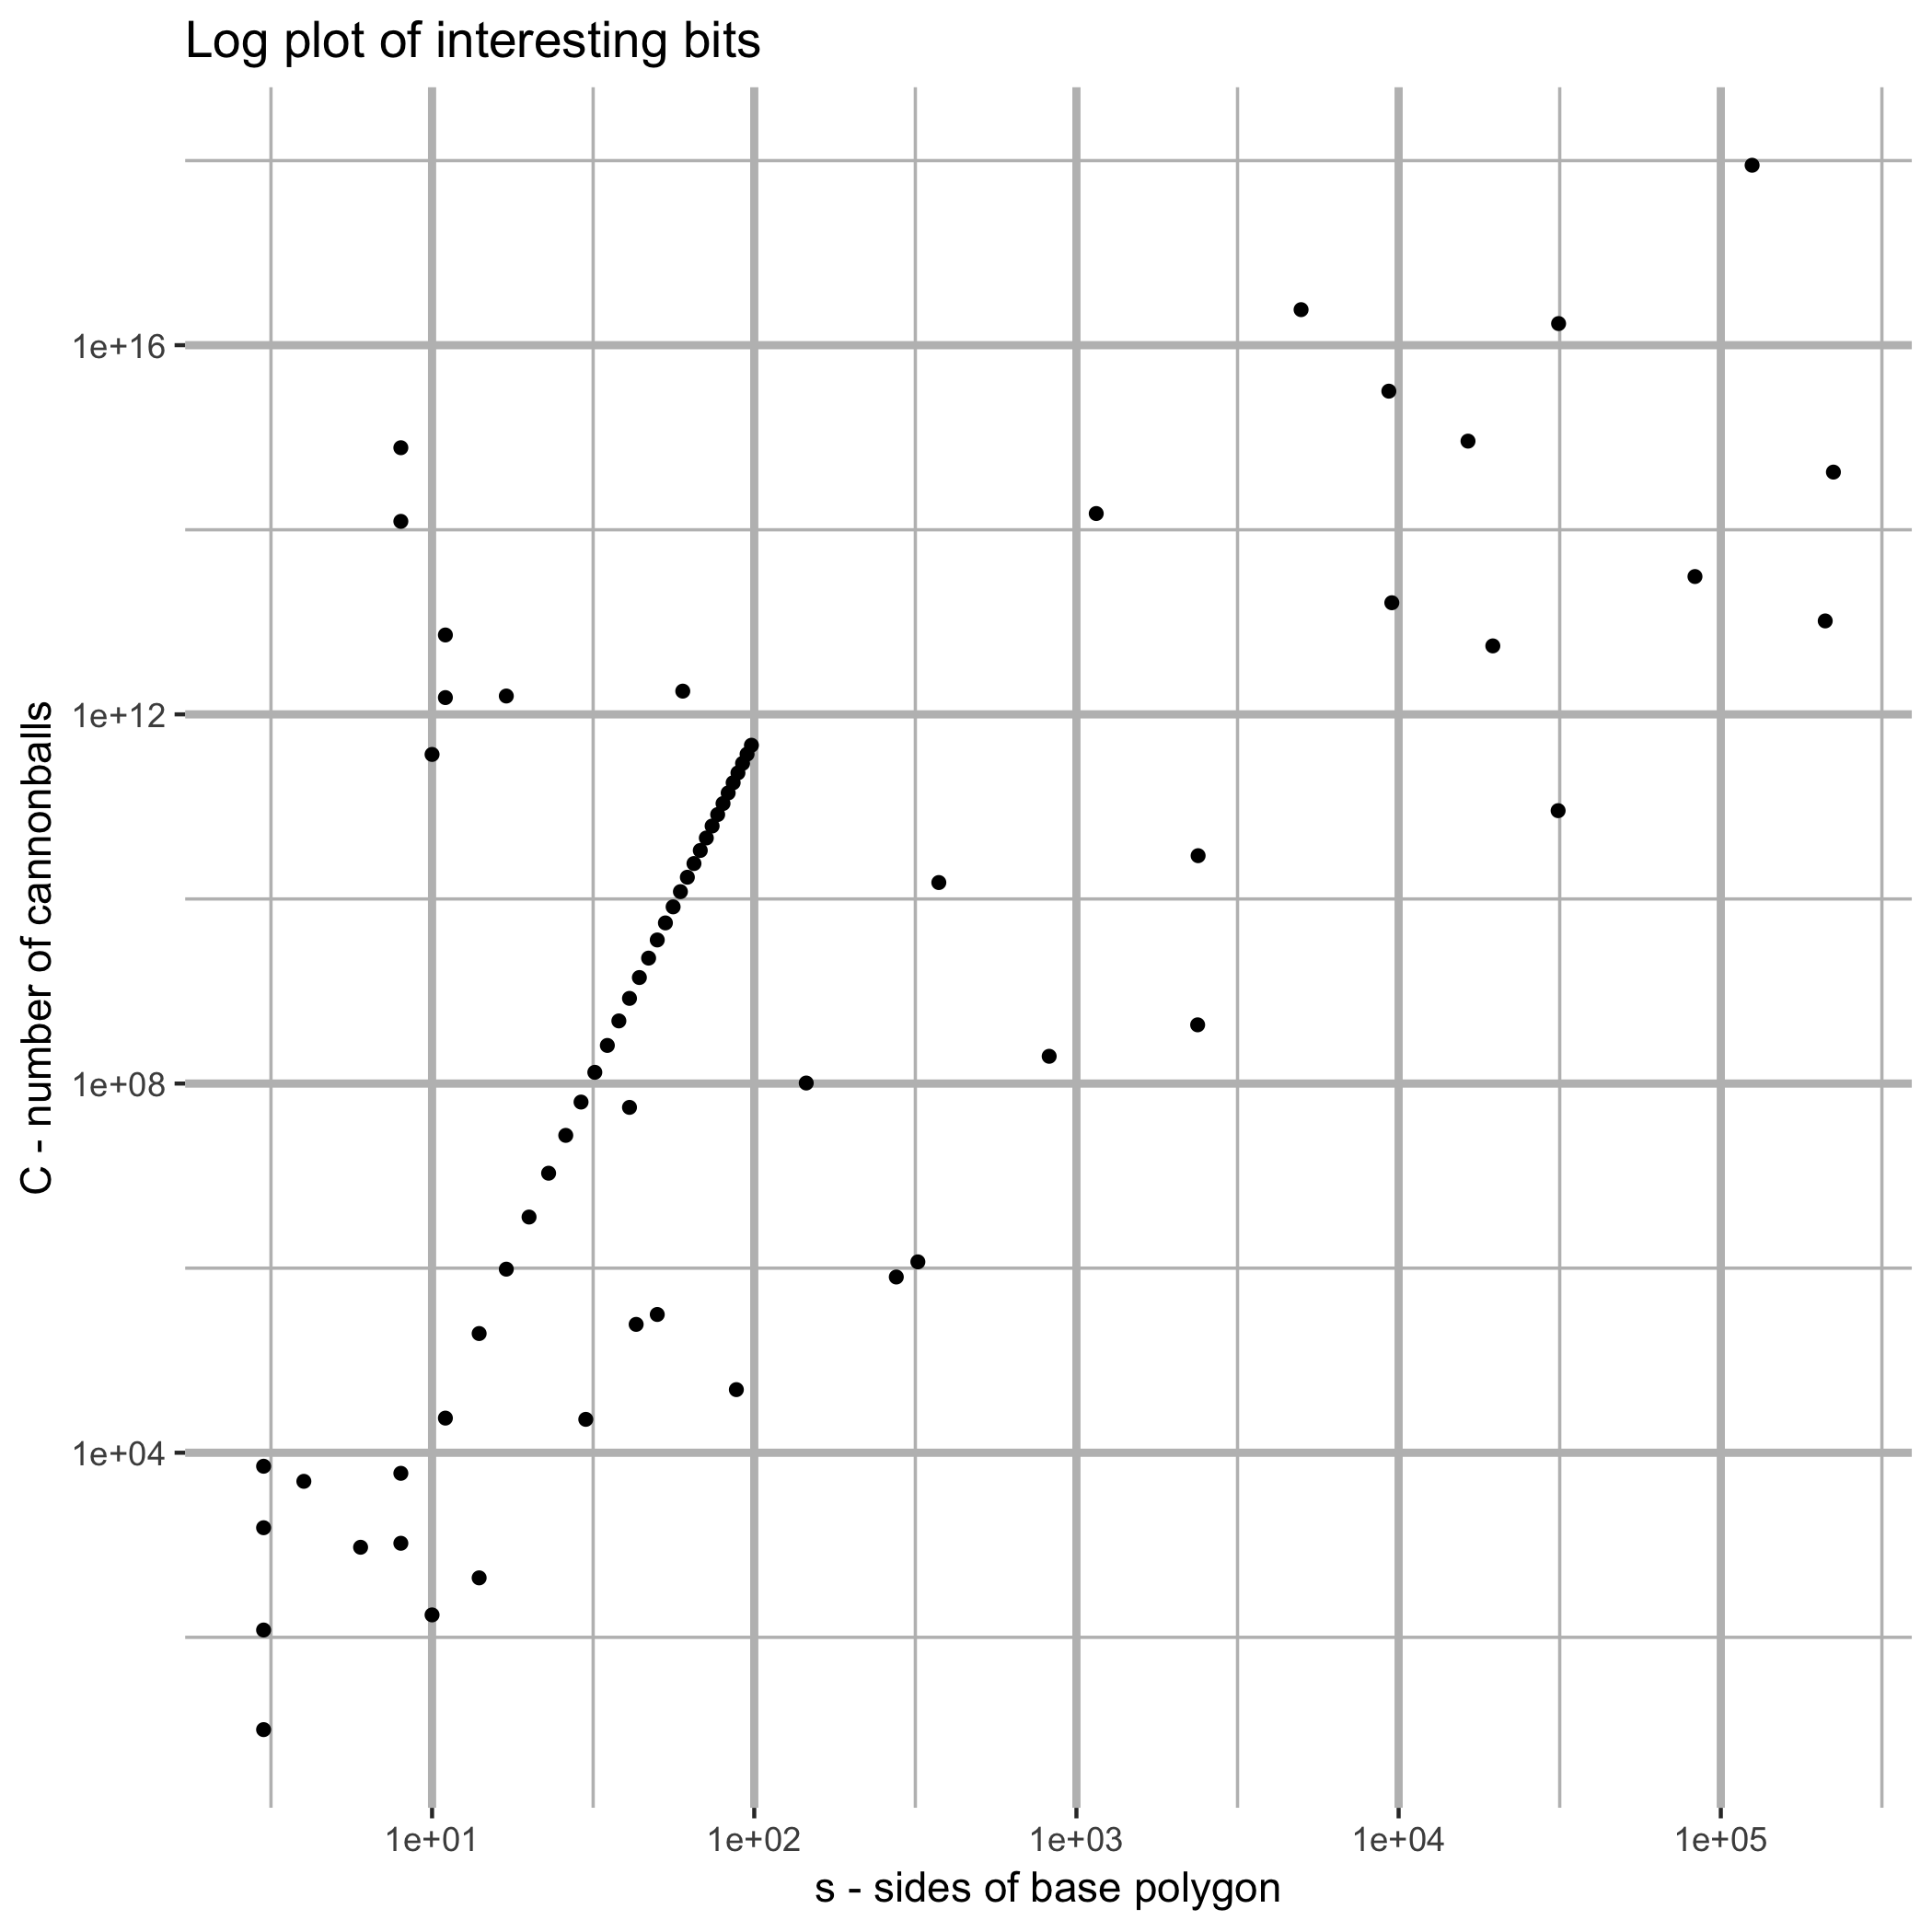
\includegraphics[width=\textwidth]{../graph/interesting_log.png}
\caption{Log plot of the remaining points}
\label{fig_log_interesting}
\end{figure}

\begin{longtable}{*4r}
\toprule
\boldmath \(s\) & \boldmath \(C(s, n_c) = P(s, n_p)\)
& \boldmath \(n_p\) & \boldmath \(n_c\) \\
\midrule
\endhead
3 & 10 & 4 & 3 \\
3 & 120 & 15 & 8 \\
3 & 1540 & 55 & 20 \\
3 & 7140 & 119 & 34 \\
4 & 4900 & 70 & 24 \\
6 & 946 & 22 & 11 \\
8 & 1045 & 19 & 10 \\
8 & 5985 & 45 & 18 \\
8 & 123395663059845 & 6413415 & 49785 \\
8 & 774611255177760 & 16068720 & 91839 \\
10 & 175 & 7 & 5 \\
10 & 368050005576 & 303336 & 6511 \\
11 & 23725 & 73 & 25 \\
11 & 1519937678700 & 581175 & 10044 \\
11 & 7248070597636 & 1269127 & 16906 \\
14 & 441 & 9 & 6 \\
14 & 195661 & 181 & 46 \\
17 & 975061 & 361 & 73 \\
17 & 1580765544996 & 459096 & 8583 \\
20 & 3578401 & 631 & 106 \\
23 & 10680265 & 1009 & 145 \\
26 & 27453385 & 1513 & 190 \\
29 & 63016921 & 2161 & 241 \\
30 & 23001 & 41 & 17 \\
32 & 132361021 & 2971 & 298 \\
35 & 258815701 & 3961 & 361 \\
38 & 477132085 & 5149 & 430 \\
41 & 55202400 & 1683 & 204 \\
41 & 837244045 & 6553 & 505 \\
43 & 245905 & 110 & 33 \\
44 & 1408778281 & 8191 & 586 \\
47 & 2286380881 & 10081 & 673 \\
50 & 314755 & 115 & 34 \\
50 & 3595928401 & 12241 & 766 \\
53 & 5501691505 & 14689 & 865 \\
56 & 8214519205 & 17443 & 970 \\
59 & 12001111741 & 20521 & 1081 \\
60 & 1785508245600 & 248132 & 5695 \\
62 & 17194450141 & 23941 & 1198 \\
65 & 24205450501 & 27721 & 1321 \\
68 & 33535911025 & 31879 & 1450 \\
71 & 45792819865 & 36433 & 1585 \\
74 & 61704091801 & 41401 & 1726 \\
77 & 82135801801 & 46801 & 1873 \\
80 & 108110983501 & 52651 & 2026 \\
83 & 140830060645 & 58969 & 2185 \\
86 & 181692979525 & 65773 & 2350 \\
88 & 48280 & 34 & 15 \\
89 & 232323110461 & 73081 & 2521 \\
92 & 294592986361 & 80911 & 2698 \\
95 & 370651946401 & 89281 & 2881 \\
98 & 462955752865 & 98209 & 3070 \\
145 & 101337426 & 1191 & 162 \\
276 & 801801 & 77 & 26 \\
322 & 1169686 & 86 & 28 \\
374 & 15064335000 & 9000 & 624 \\
823 & 197427385 & 694 & 113 \\
1152 & 149979784926720 & 510720 & 9215 \\
2378 & 432684460 & 604 & 103 \\
2386 & 29437553530 & 4970 & 420 \\
4980 & 24264913354964425 & 3122317 & 30810 \\
9325 & 3176083959788026 & 825436 & 12691 \\
9525 & 16195753597485 & 58322 & 2169 \\
16420 & 913053565546276 & 333506 & 6936 \\
19605 & 5519583702676 & 23731 & 1191 \\
31265 & 90525801730 & 2407 & 259 \\
31368 & 17147031694579605 & 1045635 & 14858 \\
83135 & 31148407558500 & 27375 & 1310 \\
125070 & 890348736143873526 & 3773306 & 34956 \\
210903 & 10290361955160 & 9879 & 664 \\
223613 & 421687634347915 & 61414 & 2245 \\

\bottomrule
\caption{Polygonal Cannonball Numbers}
\label{tab_ugly}
\end{longtable}
